\appendix
\section{APPENDIX} \label{sec:appendix_XYZ}


%\section{Code Users Manual} \label{subsec:code}
%
%The presentation of the implemented method in this chapter is structured similarly to the structure of its implementation.
%The whole implementation focuses four scripts:\begin{enumerate}
%	\item \texttt{x1\_dataset\_to\_globalAdjList.py}
%	\item \texttt{x2\_wllt\_constructor.py}
%	\item \texttt{x3\_wllt\_edge\_weight\_learning.py}
%	\item \texttt{x4\_eval\_learner.py}
%\end{enumerate}
%Some of these scripts use implementations from further files and packages, but they summarize the main steps when working with the data.
%For better orientation in the programming, we will briefly summarize these steps in advance.
%
%Independent of the origin of the dataset, it is converted in to a simple format which closely resembles the format used in the TU Dataset (\texttt{dataset\_loaders.py}).
%We call graphs in this format \textbf{general graph} and each such data structure consists of 
%\begin{itemize}
%	\item an edge set,
%	\item a vertex label dictionary and
%	\item an edge label dictionary.
%\end{itemize}
%This process can be triggered by calling the script \texttt{x1\_dataset\_to\_globalAdjList.py}. 
%It will then proceed to clean the dataset by deleting graphs with no vertices, map the given initial labels to an interval $[0, l]$ and map the indices of all graphs to a global index of the graph in the whole dataset, starting with index zero.
%The latter allows us to consider the graph dataset as one (not connected) graph, and simplifies the representation by storage in a vector.
%A directory, named after the graph dataset, is created and four essential files are stored in it.
%These files contain the whole dataset by storing an adjacency list, the graph classes, graph vertices and the original vertex labels.
%The file containing the adjacency list stores a list of indices of the neighbors of vertex $i$ (referring to the global labeling) at the $i$-th position.
%Similarly, the original vertex labels for vertex $i$ are stored at position $i$ of the respective file.
%The files containing the graph classes and vertices similarly store the class of graph $i$ and a list of all vertices that are in it ar position $i$.
%
%Given the storage path of this dataset, one can call the script \texttt{x2\_wllt\_constructor.py} to construct a WLLT on it.
%This will trigger the creation of more files, stored in a sub-directory.
%The saved WLLT consists of files all edge weights in the tree, a list of all parent vertices for every vertex (except the root) and one list for every depth of the WLLT vertex labels (WL labels) at that depth.
%On top of that, files are stored to easily access some meta information on the WLLT and its storage, to get the lowest WL label for each layer, to get the input of the hash function from which a WL label originated and to get the graph representation vectors for every graph of the dataset.
%It is possible to use the script \texttt{x2\_wllt\_constructor.py} to read-in an already constructed WLLT and add more layers to it.
%Accordingly all necessary files are updated.


%\begin{minted}{python}	
%	def custom_loss_gaussian(state, action, reward):
%	# Predict mu and sigma with actor network
%	mu, sigma = actor_network(state)
%	
%	# Compute Gaussian pdf value
%	pdf_value = tf.exp(-0.5 * ((action — mu) / (sigma))**2)
%	* 1 / (sigma * tf.sqrt(2 * np.pi))
%	
%	# Convert pdf value to log probability
%	log_probability = tf.math.log(pdf_value + 1e-5)
%	
%	# Compute weighted loss
%	loss_actor = — reward * log_probability
%	
%	return loss_actor
%\end{minted}



%		\textit{Theorem:} Isomorphy invariance of Weisfeiler and Leman's vertex representation.	Let $G, H$ be two graphs with vertex label functions $r_0^{\text{WL}, G}, r_0^{\text{WL}, H}$. If $G$ and $H$ are isomorphic (respecting $r_0^{\text{WL}, G}$, $r_0^{\text{WL}, H}$) then
%		\[ \forall k\ge 0:\qquad \mset{ r_k^{\text{WL}, G}(v)| \ v\in V(G)} =  \mset{ r_k^{\text{WL}, H}(v)| \ v\in V(H)} \]
%		%{\ref{thm:WeisfeilerLemanIsoInv}}
%		%The proof follows directly from the invariance theorem (theorem \ref{thm:MessagePassingInvariantUnderIsom}) for the message passing framework


%\subsection{Graph Dataset Hyper-graph}
%
%The separation between different graphs will only be required for classification tasks, when computing the distance between two graphs, and when computing the edge weight updates.
%
%For the implementation of the construction of the WLLT it is simpler to consider the dataset as one big disconnected hyper graph.
%\dots
%
%
%\subsection{WL Labeling Scheme}
%	The naive implementation of the WL-labeling scheme requires to aggregate the WL-labels in the neighborhood of each vertex, combine this aggregation with the WL-label of the vertex itself and hash it to obtain a new WL-label (with a perfect hash function) for the next iteration. 
%	To obtain a maximally powerful embedding, the aggregation and hashing must be injective~\cite{2019_Xu_CONF}.
%	
%	Instead of using the same set of labels (the prime numbers) for each WL labeling iteration, the WL labels were defined using a counter.
%	The counter was incremented with every new input of the hash function.
%	Additionally, the $n$ original vertex labels of the graph dataset were mapped onto the interval $[0, n-1]\in\IN$ and treated as the first outcomes of the hash function.
%	Finally, the root of the WLLT was given the artificial label of $-1$, whose convenient practical use will become clear in just a moment.
%	Now the WL counter and thus the WL labels can be set in such a way, that all $t$ WL labels in the WLLT are unique and from the interval $[-1, t-1] \in \IN$.
%	Now perform the construction of the WL labelings for the dataset in a breath-first manner, such that all WL labelings of depth $d$ are computed for all graphs in the dataset, before proceeding with depth $d+1$.
%	This way the set of all WL labels of every layer is an interval of natural numbers too.
%	The practical benefit of this is, that now every edge in the WLLT can be enumerated with numbers from $[0, t-1]$ by the WL label of its child vertex.
%	Storing all edge weights in a vector $w$ allows for a convenient access of the edge weights for label $x$ by evaluating $w[x]$.


	
%	\paragraph{Prime WL labeling}
%	This injective aggregation is often realized by sorting the WL-labels of the neighborhood first.
%	By design, the labeling scheme only requires information about the neighborhoods (adjacency matrix) and the WL-labels of the last iteration in order to compute the next WL-labels (containing information about a neighborhood or larger degree).
%	This can intuitively be understood as a recursive matrix-vector multiplication.
%	Given the fixed adjacency matrix $A\in\{0,1\}^{|V|}$, the goal is to define WL-labels (WL-features) $w_i \in \IR^{|V|}$ such that the multiplication $A w_i$ leads to the next WL-labels $w_{i+1}$.
%	This way, the new WL-labels are computed purely as an addition of the old WL-labels.
%	Using any numbers is not injective, since addiction is not an injective function.
%	One may think of prime numbers for the WL-labels, since these are at least injective with respect to multiplication.
%	To get from addiction to multiplication one can use the (injective) logarithm of prime numbers.
%	To do so, map the original $n$ vertex labels to the logarithms of the first $n$ prime numbers. 
%	With original labels given by $\ell_0:V\to[n]$ and prime numbers $p_i\in\IP$ this can be written as: 
%	\[ \forall v: \ell_0(v) \mapsto \log(p_{\ell_0(v)}) =: \ell_1(v) \]
%	Now, the $1$-th WL label can be computed as
%	\[ \ell^{\prime}_{1}(\overleftarrow{v}) := \pi\ell_{0}(\overleftarrow{v}) + A \;\ell_{0}(\overleftarrow{v}) = (A+\pi\mathbb{1}) \ell_{0}(\overleftarrow{v})\]
%	The factor $\pi$ can be replaced by any transcendent number.
%	It ensures that in the computation of the new label for a vertex $v$ the old label is differentiated from the labels of the neighborhood.
%	Consider for example a vertex with WL label $2$ and two neighboring vertices with labels $3$ each.
%	If the old labels are not differentiated from the labels of the neighborhood, the vertex with label $2$ in this example would obtain the same label as a vertex with label $3$ and two neighboring vertices with labels $2$ and $3$.
%	To ensure injectivity of the multiplication, $\ell^{\prime}_{1}$ needs to return prime numbers.
%	With each iteration the used label values are getting bigger.
%	Thus the logarithms of these values may have less and less difference, which could lead to practical problems due to the limited machine precision.
%	Thus this method works best, if for each iteration again the lowest prime numbers are used and the image of the hashes may intersect in each iteration.	
%	This intersection however makes it more tedious to keep track of the hierarchy of the WL labels, and also demands additional storage when reconstructing the unfolding tree from a WL label.
%	
%	Thus this prime number approach was discarded, and a slower more intuitive implementation was chosen.
%	The longer runtime for the used datasets is insignificant compared to the runtime for the edge weight learner anyways.	
%	\begin{algorithm}[H] FRENCH RAILWAY METRIC
%		\caption{Ground distance learning} \label{alg:GroundDistanceLearning} 
%		\begin{tabbing}
%			\textbf{Output:} \= \kill
%			\textbf{Input:} \>a graph dataset $\mathcal{G}$,\\
%			\>learning rate $\lambda$,\\
%			\>number of learning epochs $k$.\\
%			\textbf{Output:} \>Distance matrix $D$ on $\mathcal{G}$.
%		\end{tabbing}	
%		\begin{algorithmic}[1]				
%			\For {$i=0$ to $k$}
%			\For {$G_1$ and $G_2$ in $\mathcal{G}$}
%			\State $C=\operatorname{FRM}_T(G_1, G_2)$ \Comment{Ground distance computation}
%			\State $i,j = \amax{}\Big( \min\limits_{T\in\mathcal{T}} \langle T,C\rangle \Big)$ \Comment{Wasserstein distance computation} \label{alg:UpdateTarget}
%			\State $\Delta w\big(P_{i,j}\big) = \lambda \big|c(G_1)-c(G_2)\big|$ \Comment{Evaluation}\label{alg:Evaluation}
%			\State $w\big(P_{i,j}\big) = w\big(P_{i,j}\big) + \Delta  w\big(P_{i,j}\big)$ \Comment{Distance update}\label{alg:DistUpdate}
%			\EndFor
%			\EndFor
%			\State \textbf{return} $D$ with $D_{i,j} = \min\limits_{P\in\Gamma} \Big(P, \ \operatorname{FRM}_T(G_i, G_j) \Big)$ \Comment{Distance matrix on $\mathcal{G}$}
%		\end{algorithmic}
%	\end{algorithm}

%Since a successful (with respect to the research goal) implementation of the ground distance learning is yet unknown, the pseudo-code given in algorithm \ref{alg:GroundDistanceLearning} shall give a first implementation goal.
%The final procedure may be different in several aspects.
%
%There are three lines of code, which may nor may not be changed from the following initial interpretation.
%
%First, in line \ref{alg:UpdateTarget} it is denoted that the weight learning will target only the two weights which are linked to the highest cost in the optimal transport solution.
%It may be suitable to adjust all weights according to the costs of their mapping.
%
%Second, line \ref{alg:DistUpdate} aims to increase the distance between two graphs if their (binary) classes are distinct (line \ref{alg:Evaluation}).
%However, it may also be suitable to decrease their distance, if their classes are equal.
%And, a more complex update procedure may be needed, if more that two classes are present.
%Furthermore there are several ways to in- or decrease their distance.
%Before investigating methods like for example gradient descent, a fixed distance increment shall be used.
%
%Third, line \ref{alg:DistUpdate} denotes the edge weight update such that the tree distance (path weight) between the two given labels is changed.
%In general, this cannot be done, such that distances between other labels are not changed.
%But it can be done by changing all edge weights for all edges on the path (influencing a lot of other distances).
%Or by changing only the first and last edge weights (influencing only the distances concerning these two labels).
%The latter mechanism shall be investigated (first).

\subsection{WLLT Statistics} \label{Asub:WLLTStatistics}
	
	\begin{table}[!ht]
		\centering
		\begin{tabular}{|l||r|r|r|r|r||r|}
			\hline
			\textbf{} & \textbf{Layer 0} & \textbf{Layer 1} & \textbf{Layer 2} & \textbf{Layer 3} & \textbf{Layer 4} & \textbf{Sum}\\ \hline\hline
			\textbf{AIDS} & 38 & 367 & 3297 & 10298 & 15030 & 29030 \\ \hline
			\textbf{AIDS\_c} & 31 & 263 & 2419 & 7028 & 9893  & 19634 \\ \hline
			\textbf{AIDS\_perfect} & 61 & 538 & 4522 & 12310 & 16865 & 34296 \\ \hline
			\textbf{ENZYMES} & 4 & 231 & 10416 & 15208 & 16029 & 41888 \\ \hline
			\textbf{ENZYMES\_c} & 4 & 229 & 10414 & 15206 & 16027 & 41880 \\ \hline
			\textbf{MSRC\_9} & 11 & 2053 & 8632 & 8929 & 8929 & 28554 \\ \hline
			\textbf{MSRC\_21} & 23 & 7736 & 40547 & 43470 & 43489 & 135265 \\ \hline
			\textbf{MSRC\_21C} & 22 & 3551 & 8312 & 8382 & 8382 & 28649 \\ \hline
			\textbf{MUTAG} & 7 & 33 & 174 & 572 & 1197 & 1983 \\ \hline
			\textbf{NCI1} & 38 & 292 & 4058 & 22948 & 44508 & 71844 \\ \hline
			\textbf{ogbg-molbace} & 74 & 1425 & 5588 & 10540 & 15228 & 32855 \\ \hline
			\textbf{ogbg-molbbbp} & 95 & 4221 & 15373 & 24581 & 30407 & 74677 \\ \hline
			\textbf{PROTEINS} & 4 & 297 & 20962 & 35676 & 37940 & 94879 \\ \hline
			\textbf{PROTEINS\_c} & 4 & 296 & 20764 & 35176 & 37369 & 93609 \\ \hline
			\textbf{PTC\_MR} & 19 & 130 & 780 & 1987 & 2803 & 5719 \\ \hline
			\textbf{Tox21\_AHR} & 50 & 432 & 4325 & 22012 & 43112 & 69931 \\ \hline
		\end{tabular}
		\caption{WLLT sizes for different datasets. See section \ref{subsec:datasets} for more information on the datasets.}
		\label{tab:WLLTsize}
	\end{table}
	See figures \ref{fig:wlltstatstuds}, \ref{fig:wlltstatsogbds}, and \ref{fig:wlltstatsallds} for visualizations of the table \ref{tab:WLLTsize}.
		
		
	\begin{figure}[H]
		\centering
		\begin{subfigure}{0.45\textwidth}
			\centering
			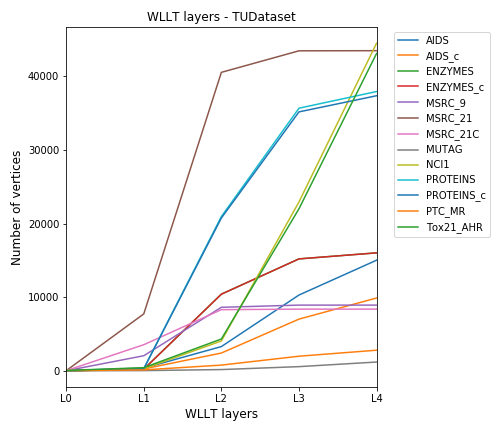
\includegraphics[width=1.\linewidth]{images/WLLTstats_TUDs}
			\caption{TUDatasets.}
			\label{fig:wlltstatstuds}
		\end{subfigure}
		\begin{subfigure}{0.45\textwidth}
			\centering
			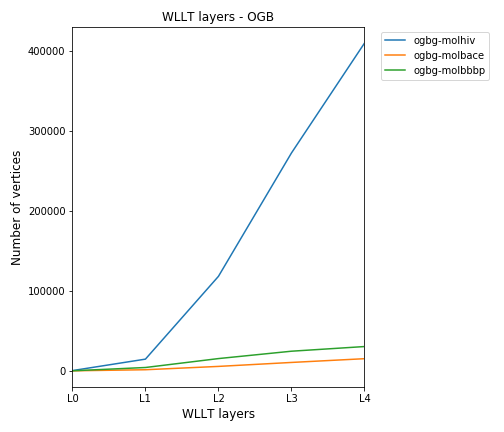
\includegraphics[width=1.\linewidth]{images/WLLTstats_OgbDs}
			\caption{OGB datasets.}
			\label{fig:wlltstatsogbds}
		\end{subfigure}
		\caption{Figure \ref{fig:wlltstatsallds} divided by dataset collection.}
		\label{fig:wlltstatstudsandogbds}
	\end{figure}
	
\subsection{Weisfeiler Lehman Kernel on TUDatasets}\label{Appendix:FurtherResults}

\begin{figure}[H]
	\centering
	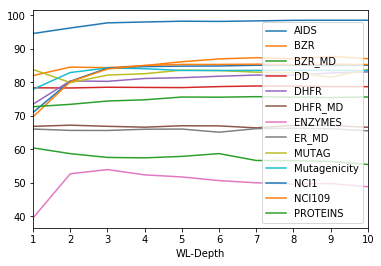
\includegraphics[width=0.7\linewidth]{images/plot_TUDataset_Benchmarks}
	\caption{TUDataset - SVM accuracies.}
	\label{fig:SVM_WL_TUDatasets}
\end{figure}

\subsection{Overview Graph Kernel Methods} \label{Asub:SVMacc}
	The following table presents more SVM accuracies of the l-WWLLT Kernel for different configurations and datasets.
	For all these configurations, the push- and pull-factors are applied in a multiplicative way and the edge weights are limited to the interval $[0,2]$.
%	\begin{landscape}
	\begin{longtable}{|l||r|r|r|r|r|r||r|r|}
		\hline
		\textbf{Dataset} & $D$ & $lr$ & $bs_p$ & $f_{\text{pull}}$ & $f_{\text{push}}$ & $t_{\text{he}}$ & \textbf{SVM} & E \\ \hline\hline
		\textbf{AIDS} & 9 & 1.00 & 0.05 & 0.50 & 0.50 & 1.00 & 80.00 & 0 \\ \hline
		\textbf{AIDS} & 4 & 0.20 & 0.05 & 0.30 & 0.20 & 0.30 & 96.57 & 0 \\ \hline
		\textbf{AIDS} & 4 & 0.20 & 0.10 & 0.30 & 0.20 & 0.30 & 96.48 & 0 \\ \hline
		\textbf{AIDS} & 4 & 0.50 & 0.05 & 0.30 & 0.20 & 0.30 & 96.43 & 0 \\ \hline
		\textbf{AIDS} & 2 & 0.50 & 0.05 & 0.30 & 0.20 & 0.30 & 98.57 & 1 \\ \hline
		\textbf{AIDS} & 4 & 0.50 & 0.05 & 0.30 & 0.20 & 0.30 & 96.46 & 0 \\ \hline
		\textbf{AIDS} & 4 & 0.80 & 0.05 & 0.50 & 0.50 & 1.00 & 97.28 & 9 \\ \hline
		\textbf{AIDS} & 4 & 0.80 & 0.05 & 0.50 & 0.50 & 1.00 & 97.24 & 9 \\ \hline
		\textbf{AIDS} & 4 & 0.80 & 0.05 & 0.50 & 0.50 & 1.00 & 97.49 & 9 \\ \hline
		\textbf{AIDS} & 4 & 0.80 & 0.05 & 0.20 & 0.20 & 0.60 & 97.29 & 10 \\ \hline
		\textbf{AIDS} & 4 & 0.80 & 0.05 & 0.40 & 0.10 & 1.00 & 96.50 & 0 \\ \hline
		\textbf{AIDS} & 4 & 1.00 & 0.10 & 0.30 & 0.05 & 1.00 & 96.51 & 0 \\ \hline
		\textbf{AIDS} & 4 & 1.00 & 0.05 & 0.40 & 0.40 & 1.00 & 97.32 & 9 \\ \hline
		\textbf{AIDS} & 4 & 0.80 & 0.05 & 0.50 & 0.50 & 1.00 & 97.27 & 10 \\ \hline
		\textbf{AIDS} & 4 & 0.80 & 0.05 & 0.50 & 0.50 & 1.00 & 97.45 & 8 \\ \hline
		\textbf{AIDS} & 4 & 0.80 & 0.05 & 0.10 & 0.10 & 0.60 & 97.24 & 10 \\ \hline
		\textbf{AIDS} & 4 & 0.80 & 0.05 & 0.40 & 0.40 & 0.60 & 97.38 & 9 \\ \hline
		\textbf{AIDS} & 4 & 0.80 & 0.05 & 0.10 & 0.20 & 1.00 & 97.67 & 6 \\ \hline
		\textbf{AIDS} & 4 & 1.00 & 0.10 & 0.20 & 0.20 & 1.00 & 96.48 & 4 \\ \hline
		\textbf{AIDS} & 4 & 1.00 & 0.10 & 0.20 & 0.20 & 1.00 & 97.34 & 10 \\ \hline
		\textbf{AIDS} & 4 & 0.10 & 0.05 & 0.30 & 0.30 & 0.90 & 96.89 & 7 \\ \hline
		\textbf{AIDS} & 4 & 0.20 & 0.05 & 0.30 & 0.30 & 0.90 & 97.18 & 10 \\ \hline
		\textbf{AIDS} & 4 & 0.30 & 0.05 & 0.30 & 0.30 & 0.90 & 97.22 & 8 \\ \hline
		\textbf{AIDS} & 4 & 0.40 & 0.05 & 0.30 & 0.30 & 0.90 & 97.28 & 7 \\ \hline
		\textbf{AIDS} & 4 & 0.50 & 0.05 & 0.30 & 0.30 & 0.90 & 97.28 & 10 \\ \hline
		\textbf{AIDS} & 4 & 0.60 & 0.05 & 0.30 & 0.30 & 0.90 & 97.28 & 8 \\ \hline
		\textbf{AIDS} & 4 & 0.70 & 0.05 & 0.30 & 0.30 & 0.90 & 97.34 & 9 \\ \hline
		\textbf{AIDS} & 4 & 1.00 & 0.05 & 0.40 & 0.40 & 1.00 & 80.00 & 0 \\ \hline
		\textbf{AIDS} & 4 & 1.00 & 0.05 & 0.40 & 0.40 & 1.00 & 80.00 & 0 \\ \hline
		\textbf{AIDS} & 4 & 1.00 & 0.05 & 1.00 & 0.80 & 1.00 & 80.00 & 0 \\ \hline
		\textbf{AIDS} & 4 & 1.00 & 0.05 & 0.30 & 0.10 & 0.60 & 80.00 & 0 \\ \hline
		\textbf{AIDS} & 4 & 1.00 & 0.05 & 0.50 & 0.50 & 0.60 & 80.00 & 0 \\ \hline
		\textbf{AIDS} & 4 & 1.00 & 0.05 & 0.10 & 0.30 & 0.60 & 80.00 & 0 \\ \hline
		\textbf{AIDS} & 4 & 1.00 & 0.05 & 0.30 & 0.10 & 0.60 & 80.00 & 0 \\ \hline
		\textbf{AIDS} & 4 & 1.00 & 0.05 & 0.50 & 0.50 & 1.00 & 96.48 & 0 \\ \hline
		\textbf{AIDS} & 4 & 1.00 & 0.05 & 0.50 & 0.50 & 1.00 & 96.46 & 0 \\ \hline
		\textbf{AIDS} & 4 & 1.00 & 0.05 & 0.50 & 0.50 & 1.00 & 96.38 & 0 \\ \hline
		\textbf{AIDS} & 4 & 0.80 & 0.05 & 0.30 & 0.30 & 0.90 & 97.37 & 10 \\ \hline
		\textbf{AIDS} & 4 & 1.00 & 0.05 & 0.10 & 0.05 & 0.90 & 96.39 & 0 \\ \hline
		\textbf{AIDS} & 4 & 0.80 & 0.05 & 0.30 & 0.30 & 0.90 & 97.33 & 10 \\ \hline
		\textbf{AIDS} & 4 & 0.90 & 0.05 & 0.30 & 0.30 & 0.90 & 97.40 & 9 \\ \hline
		\textbf{AIDS} & 4 & 1.00 & 0.05 & 0.30 & 0.30 & 0.90 & 97.45 & 10 \\ \hline
		\textbf{AIDS} & 9 & 1.00 & 0.05 & 0.50 & 0.50 & 1.00 & 80.00 & 0 \\ \hline
		\textbf{AIDS} & 9 & 1.00 & 0.05 & 0.50 & 0.50 & 1.00 & 80.00 & 0 \\ \hline
		\textbf{AIDS} & 9 & 1.00 & 0.05 & 0.50 & 0.50 & 1.00 & 80.00 & 0 \\ \hline
		\textbf{AIDS} & 4 & 1.00 & 0.05 & 1.00 & 0.10 & 1.00 & 80.00 & 0 \\ \hline
		\textbf{AIDS} & 4 & 1.00 & 0.05 & 0.50 & 0.10 & 1.00 & 80.00 & 0 \\ \hline
		\textbf{AIDS} & 4 & 1.00 & 0.05 & 0.10 & 1.00 & 1.00 & 80.00 & 0 \\ \hline
		\textbf{AIDS} & 4 & 1.00 & 0.05 & 0.10 & 0.10 & 1.00 & 80.00 & 0 \\ \hline
		\textbf{AIDS} & 4 & 1.00 & 0.05 & 0.50 & 0.50 & 1.00 & 80.00 & 0 \\ \hline
		\textbf{AIDS} & 4 & 1.00 & 0.05 & 1.00 & 1.00 & 1.00 & 80.00 & 0 \\ \hline
		\textbf{AIDS\_c} & 4 & 1.00 & 0.05 & 0.10 & 0.10 & 0.60 & 97.10 & 0 \\ \hline
		\textbf{AIDS\_c} & 4 & 1.00 & 0.05 & 0.50 & 0.50 & 0.60 & 97.51 & 0 \\ \hline
		\textbf{AIDS\_c} & 4 & 1.00 & 0.05 & 1.00 & 1.00 & 0.60 & 97.54 & 0 \\ \hline
		\textbf{AIDS\_c} & 4 & 1.00 & 0.05 & 1.00 & 0.10 & 1.00 & 96.65 & 0 \\ \hline
		\textbf{AIDS\_c} & 4 & 1.00 & 0.05 & 0.10 & 0.50 & 1.00 & 97.75 & 10 \\ \hline
%				\textbf{AIDS\_perfect} & 4 & 1.00 & 0.05 & 0.10 & 0.10 & 0.60 & 99.49 & 0 \\ \hline
%				\textbf{AIDS\_perfect} & 4 & 1.00 & 0.05 & 0.30 & 0.10 & 0.60 & 98.40 & 1 \\ \hline
%				\textbf{AIDS\_perfect} & 4 & 1.00 & 0.2 & 0.30 & 0.10 & 0.60 & 98.34 & 5 \\ \hline
%				\textbf{AIDS\_perfect} & 2 & 1.00 & 0.05 & 0.30 & 0.10 & 0.60 & 98.36 & 1 \\ \hline
%				\textbf{AIDS\_perfect} & 2 & 1.00 & 0.05 & 0.30 & 0.10 & 0.30 & 98.93 & 6 \\ \hline
%				\textbf{AIDS\_perfect} & 4 & 1.00 & 0.05 & 0.30 & 0.10 & 0.60 & 98.98 & 8 \\ \hline
%				\textbf{AIDS\_SeparateClusters} & 4 & 1.00 & 0.21 & 0.40 & 0.40 & 1.00 & 87.80 & 10 \\ \hline
%				\textbf{AIDS\_SeparateClusters} & 4 & 1.00 & 0.21 & 0.40 & 0.40 & 1.00 & 86.80 & 0 \\ \hline
%				\textbf{AIDS\_SeparateClusters} & 4 & 1.00 & 0.21 & 0.40 & 0.40 & 1.00 & 85.20 & 6 \\ \hline
%				\textbf{AIDS\_SeparateClusters} & 4 & 1.00 & 0.21 & 0.40 & 0.40 & 1.00 & 88.40 & 3 \\ \hline
%				\textbf{AIDS\_SeparateClusters} & 4 & 1.00 & 0.21 & 0.40 & 0.40 & 1.00 & 87.00 & 10 \\ \hline
		\textbf{ENZYMES} & 4 & 1.00 & 0.05 & 0.10 & 0.10 & 0.60 & 54.38 & 4 \\ \hline
		\textbf{ENZYMES} & 4 & 1.00 & 0.05 & 0.50 & 0.50 & 0.60 & 54.67 & 10 \\ \hline
		\textbf{ENZYMES} & 4 & 1.00 & 0.05 & 1.00 & 1.00 & 0.60 & 54.40 & 9 \\ \hline
		\textbf{ENZYMES} & 4 & 1.00 & 0.05 & 1.00 & 0.10 & 1.00 & 53.75 & 0 \\ \hline
		\textbf{ENZYMES} & 4 & 1.00 & 0.05 & 0.10 & 0.50 & 1.00 & 59.43 & 7 \\ \hline
		\textbf{ENZYMES\_c} & 4 & 1.00 & 0.05 & 0.10 & 0.10 & 0.60 & 54.15 & 7 \\ \hline
		\textbf{ENZYMES\_c} & 4 & 1.00 & 0.05 & 0.50 & 0.50 & 0.60 & 54.24 & 4 \\ \hline
		\textbf{ENZYMES\_c} & 4 & 1.00 & 0.05 & 1.00 & 1.00 & 0.60 & 54.10 & 1 \\ \hline
		\textbf{ENZYMES\_c} & 4 & 1.00 & 0.05 & 1.00 & 0.10 & 1.00 & 52.69 & 0 \\ \hline
		\textbf{ENZYMES\_c} & 4 & 1.00 & 0.05 & 0.10 & 0.50 & 1.00 & 59.06 & 9 \\ \hline
		\textbf{MSRC\_9} & 4 & 1.00 & 0.3 & 0.20 & 0.20 & 1.00 & 91.01 & 10 \\ \hline
		\textbf{MSRC\_9} & 4 & 1.00 & 0.3 & 0.20 & 0.20 & 1.00 & 90.83 & 3 \\ \hline
		\textbf{MSRC\_9} & 4 & 1.00 & 0.3 & 0.10 & 0.10 & 0.60 & 90.87 & 6 \\ \hline
		\textbf{MSRC\_9} & 4 & 1.00 & 0.3 & 0.40 & 0.40 & 0.60 & 90.87 & 5 \\ \hline
		\textbf{MSRC\_9} & 4 & 1.00 & 0.3 & 0.40 & 0.10 & 1.00 & 90.63 & 1 \\ \hline
		\textbf{MSRC\_9} & 4 & 1.00 & 0.3 & 0.10 & 0.40 & 1.00 & 90.81 & 2 \\ \hline
		\textbf{MSRC\_9} & 4 & 1.00 & 0.3 & 0.10 & 0.40 & 1.00 & 91.05 & 2 \\ \hline
		\textbf{MSRC\_9} & 4 & 1.00 & 0.3 & 0.10 & 0.40 & 1.00 & 91.01 & 2 \\ \hline
		\textbf{MSRC\_9} & 4 & 1.00 & 0.3 & 0.30 & 0.05 & 1.00 & 90.60 & 0 \\ \hline
		\textbf{MSRC\_9} & 4 & 1.00 & 0.3 & 0.20 & 0.20 & 1.00 & 90.95 & 9 \\ \hline
		\textbf{MSRC\_9} & 4 & 1.00 & 0.3 & 0.20 & 0.20 & 1.00 & 91.01 & 3 \\ \hline
		\textbf{MSRC\_9} & 2 & 1.00 & 0.3 & 0.20 & 0.20 & 1.00 & 90.83 & 0 \\ \hline
		\textbf{MSRC\_21} & 4 & 1.00 & 0.3 & 0.20 & 0.20 & 1.00 & 85.36 & 10 \\ \hline
		\textbf{MSRC\_21} & 4 & 1.00 & 0.3 & 0.20 & 0.20 & 1.00 & 87.58 & 8 \\ \hline
		\textbf{MUTAG} & 1 & 1.00 & 0.05 & 0.01 & 0.01 & 1.00 & 87.13 & 8 \\ \hline
		\textbf{MUTAG} & 1 & 1.00 & 0.05 & 0.80 & 0.80 & 1.00 & 86.66 & 4 \\ \hline
		\textbf{MUTAG} & 1 & 1.00 & 0.05 & 0.01 & 0.01 & 1.00 & 87.33 & 8 \\ \hline
		\textbf{MUTAG} & 1 & 1.00 & 0.05 & 0.01 & 0.01 & 1.00 & 87.25 & 2 \\ \hline
		\textbf{MUTAG} & 1 & 1.00 & 0.5 & 1.00 & 1.00 & 0.90 & 86.90 & 8 \\ \hline
		\textbf{MUTAG} & 4 & 1.00 & 0.2 & 0.80 & 0.80 & 0.90 & 66.51 & 10 \\ \hline
		\textbf{MUTAG} & 4 & 1.00 & 0.2 & 0.80 & 0.80 & 0.90 & 66.51 & 0 \\ \hline
		\textbf{MUTAG} & 4 & 1.00 & 0.2 & 0.30 & 0.10 & 0.60 & 66.53 & 0 \\ \hline
		\textbf{NCI1} & 4 & 1.00 & 0.05 & 0.10 & 0.10 & 0.60 & 76.65 & 10 \\ \hline
		\textbf{NCI1} & 4 & 1.00 & 0.05 & 0.30 & 0.30 & 1.00 & 76.83 & 10 \\ \hline
		\textbf{NCI1} & 4 & 1.00 & 0.05 & 0.10 & 0.50 & 1.00 & 79.44 & 10 \\ \hline
		\textbf{NCI1} & 4 & 1.00 & 0.05 & 0.50 & 0.50 & 0.60 & 77.26 & 10 \\ \hline
		\textbf{NCI1} & 4 & 1.00 & 0.05 & 1.00 & 1.00 & 0.60 & 77.63 & 10 \\ \hline
		\textbf{NCI1} & 4 & 1.00 & 0.05 & 1.00 & 0.10 & 1.00 & 76.57 & 0 \\ \hline
		\textbf{NCI1} & 4 & 1.00 & 0.05 & 0.10 & 0.10 & 1.00 & 76.66 & 8 \\ \hline
		\textbf{NCI1} & 4 & 1.00 & 0.05 & 0.30 & 0.30 & 1.00 & 76.88 & 9 \\ \hline
		\textbf{ogbg-molbace} & 4 & 1.00 & 100 & 0.20 & 0.20 & 1.00 & 82.12 & 9 \\ \hline
		\textbf{ogbg-molbace} & 4 & 1.00 & 100 & 0.10 & 0.10 & 0.60 & 81.88 & 9 \\ \hline
		\textbf{ogbg-molbace} & 4 & 1.00 & 100 & 0.40 & 0.40 & 0.60 & 82.04 & 9 \\ \hline
		\textbf{ogbg-molbace} & 4 & 1.00 & 100 & 0.40 & 0.10 & 1.00 & 81.46 & 0 \\ \hline
		\textbf{ogbg-molbace} & 4 & 1.00 & 100 & 0.10 & 0.40 & 1.00 & 83.07 & 5 \\ \hline
		\textbf{ogbg-molbace} & 4 & 1.00 & 100 & 0.30 & 0.05 & 1.00 & 81.57 & 0 \\ \hline
		\textbf{ogbg-molbace} & 4 & 1.00 & 100 & 0.20 & 0.20 & 1.00 & 81.81 & 0 \\ \hline
		\textbf{ogbg-molbace} & 4 & 1.00 & 100 & 0.20 & 0.20 & 1.00 & 82.18 & 10 \\ \hline
		\textbf{ogbg-molbace} & 2 & 1.00 & 100 & 0.20 & 0.20 & 1.00 & 83.56 & 8 \\ \hline
		\textbf{ogbg-molbbbp} & 4 & 1.00 & 100 & 0.20 & 0.20 & 1.00 & 84.30 & 10 \\ \hline
		\textbf{PROTEINS} & 4 & 1.00 & 0.05 & 0.10 & 0.10 & 0.60 & 73.22 & 10 \\ \hline
		\textbf{PROTEINS} & 4 & 1.00 & 0.05 & 0.50 & 0.50 & 0.60 & 73.50 & 6 \\ \hline
		\textbf{PROTEINS} & 4 & 1.00 & 0.05 & 1.00 & 1.00 & 0.60 & 73.57 & 4 \\ \hline
		\textbf{PROTEINS} & 4 & 1.00 & 0.05 & 1.00 & 0.10 & 1.00 & 72.49 & 0 \\ \hline
		\textbf{PROTEINS} & 4 & 1.00 & 0.05 & 0.10 & 0.50 & 1.00 & 73.81 & 10 \\ \hline
		\textbf{PROTEINS\_c} & 4 & 1.00 & 0.05 & 0.10 & 0.10 & 0.60 & 72.61 & 7 \\ \hline
		\textbf{PROTEINS\_c} & 4 & 1.00 & 0.05 & 0.50 & 0.50 & 0.60 & 72.81 & 6 \\ \hline
		\textbf{PROTEINS\_c} & 4 & 1.00 & 0.05 & 1.00 & 1.00 & 0.60 & 72.87 & 8 \\ \hline
		\textbf{PROTEINS\_c} & 4 & 1.00 & 0.05 & 1.00 & 0.10 & 1.00 & 72.52 & 0 \\ \hline
		\textbf{PROTEINS\_c} & 4 & 1.00 & 0.05 & 0.10 & 0.50 & 1.00 & 72.56 & 10 \\ \hline
		\textbf{PTC\_MR} & 4 & 1.00 & 0.3 & 0.20 & 0.20 & 1.00 & 64.59 & 4 \\ \hline
		\textbf{PTC\_MR} & 4 & 1.00 & 0.3 & 0.20 & 0.20 & 1.00 & 64.41 & 10 \\ \hline
		\textbf{PTC\_MR} & 4 & 1.00 & 0.3 & 0.20 & 0.20 & 1.00 & 64.72 & 10 \\ \hline
		\textbf{PTC\_MR} & 4 & 1.00 & 0.3 & 0.10 & 0.10 & 0.60 & 63.87 & 6 \\ \hline
		\textbf{PTC\_MR} & 4 & 1.00 & 0.3 & 0.40 & 0.40 & 0.60 & 64.92 & 1 \\ \hline
		\textbf{Tox21\_AHR} & 4 & 1.00 & 0.01 & 0.10 & 0.10 & 0.60 & 88.37 & 0 \\ \hline
	\end{longtable}		
%	\end{landscape}

%	\begin{table}[h]
%		\centering
%		\begin{tabular}{|l|l|l|l|l|l|l|l|l|l|l|l|l|l|l|}
%			\hline
%			\textbf{Dataset} & \textbf{NoG} & \textbf{sp} & \textbf{WL Avg. Acc.} & \textbf{bpsf} & \textbf{Std WL Depth 1} & \textbf{Std WL Depth 2} & \textbf{Std WL Depth 3} & \textbf{Std WL Depth 4} & \textbf{Std WL Depth 5} & \textbf{Std WL Depth 6} & \textbf{Std WL Depth 7} & \textbf{Std WL Depth 8} & \textbf{Std WL Depth 9} & \textbf{Std WL Depth 10} \\ \hline
%			AIDS & ~ & ~ & 98.7 & ~ & 94.58 & 96.22 & 97.76 & 98.02 & 98.25 & 98.19 & 98.34 & 98.52 & 98.54 & 98.54 \\ \hline
%			BZR & 86.16 & ~ & ~ & ~ & 82.02 & 84.55 & 84.39 & 85.01 & 86.15 & 86.99 & 87.36 & 87.01 & 87.73 & 87.07 \\ \hline
%			BZR+AF8-MD & ~ & ~ & 60.75 & ~ & 60.43 & 58.71 & 57.58 & 57.45 & 57.89 & 58.72 & 56.67 & 56.62 & 56.39 & 55.47 \\ \hline
%			COIL+AC0-DEL & 14.13 & ~ & ~ & ~ & ~ & ~ & ~ & ~ & ~ & ~ & ~ & ~ & ~ & ~ \\ \hline
%			COIL+AC0-RAG & 7.22 & ~ & ~ & ~ & ~ & ~ & ~ & ~ & ~ & ~ & ~ & ~ & ~ & ~ \\ \hline
%			COX2 & 81.37 & ~ & ~ & ~ & ~ & ~ & ~ & ~ & ~ & ~ & ~ & ~ & ~ & ~ \\ \hline
%			COX2+AF8-MD & 65.26 & ~ & ~ & ~ & ~ & ~ & ~ & ~ & ~ & ~ & ~ & ~ & ~ & ~ \\ \hline
%			DD & 76.67 & ~ & ~ & ~ & 78.37 & 78.32 & 78.54 & 78.48 & 78.43 & 78.73 & 78.91 & 78.88 & 78.73 & 78.7 \\ \hline
%			DHFR & ~ & ~ & 82.02 & ~ & 73.5 & 80.42 & 80.3 & 81.15 & 81.39 & 81.82 & 82.17 & 82.17 & 82.77 & 83.12 \\ \hline
%			DHFR+AF8-MD & ~ & 69.2 & ~ & ~ & 66.85 & 67.21 & 66.87 & 66.61 & 67.04 & 67 & 66.4 & 67.17 & 67.12 & 66.58 \\ \hline
%			ENZYMES & ~ & ~ & 50.67 & ~ & 39.52 & 52.7 & 53.95 & 52.37 & 51.75 & 50.67 & 50 & 49.62 & 49.78 & 48.83 \\ \hline
%			ER+AF8-MD & 74.46 & ~ & ~ & ~ & 66.06 & 65.65 & 65.63 & 66 & 66.05 & 65.11 & 66.18 & 66.31 & 66.14 & 65.53 \\ \hline
%			IMDB+AC0-BINARY & 70.7 & ~ & ~ & ~ & ~ & ~ & ~ & ~ & ~ & ~ & ~ & ~ & ~ & ~ \\ \hline
%			IMDB+AC0-MULTI & 46.73 & ~ & ~ & ~ & ~ & ~ & ~ & ~ & ~ & ~ & ~ & ~ & ~ & ~ \\ \hline
%			Letter+AC0-high & 34.58 & ~ & ~ & ~ & ~ & ~ & ~ & ~ & ~ & ~ & ~ & ~ & ~ & ~ \\ \hline
%			Letter+AC0-low & 48.6 & ~ & ~ & ~ & ~ & ~ & ~ & ~ & ~ & ~ & ~ & ~ & ~ & ~ \\ \hline
%			Letter+AC0-med & ~ & 44.67 & ~ & ~ & ~ & ~ & ~ & ~ & ~ & ~ & ~ & ~ & ~ & ~ \\ \hline
%			MSRC+AF8-21 & 86.46 & ~ & ~ & ~ & ~ & ~ & ~ & ~ & ~ & ~ & ~ & ~ & ~ & ~ \\ \hline
%			MSRC+AF8-21C & 81.59 & ~ & ~ & ~ & ~ & ~ & ~ & ~ & ~ & ~ & ~ & ~ & ~ & ~ \\ \hline
%			MSRC+AF8-9 & 88.35 & ~ & ~ & ~ & ~ & ~ & ~ & ~ & ~ & ~ & ~ & ~ & ~ & ~ \\ \hline
%			MUTAG & 87.31 & ~ & ~ & ~ & 83.83 & 79.92 & 82.16 & 82.58 & 83.63 & 83.51 & 83.04 & 82.92 & 81.54 & 83.85 \\ \hline
%			Mutagenicity & ~ & ~ & 83.56 & ~ & 77.91 & 82.93 & 84.3 & 84.07 & 83.55 & 83.54 & 83.57 & 83.58 & 83.54 & 83.53 \\ \hline
%			NCI1 & ~ & ~ & 84.72 & ~ & 71.02 & 80.31 & 84.23 & 84.71 & 84.84 & 84.89 & 85.1 & 85.09 & 85.05 & 85.13 \\ \hline
%			NCI109 & ~ & ~ & 85.2 & ~ & 69.73 & 80.17 & 83.99 & 85.04 & 85.35 & 85.35 & 85.42 & 85.32 & 85.42 & 85.32 \\ \hline
%			PROTEINS & 74.58 & ~ & ~ & ~ & 72.72 & 73.43 & 74.42 & 74.79 & 75.61 & 75.57 & 75.72 & 75.56 & 75.47 & 75.63 \\ \hline
%			PROTEINS+AF8-full & 74.58 & ~ & ~ & ~ & ~ & ~ & ~ & ~ & ~ & ~ & ~ & ~ & ~ & ~ \\ \hline
%			PTC+AF8-FM & 63.63 & ~ & ~ & ~ & ~ & ~ & ~ & ~ & ~ & ~ & ~ & ~ & ~ & ~ \\ \hline
%			PTC+AF8-FR & 67.25 & ~ & ~ & ~ & ~ & ~ & ~ & ~ & ~ & ~ & ~ & ~ & ~ & ~ \\ \hline
%			PTC+AF8-MM & 66.7 & ~ & ~ & ~ & ~ & ~ & ~ & ~ & ~ & ~ & ~ & ~ & ~ & ~ \\ \hline
%			PTC+AF8-MR & 57.6 & ~ & ~ & ~ & ~ & ~ & ~ & ~ & ~ & ~ & ~ & ~ & ~ & ~ \\ \hline
%			REDDIT+AC0-BINARY & 82.5 & ~ & 72.8 & ~ & ~ & ~ & ~ & ~ & ~ & ~ & ~ & ~ & ~ & ~ \\ \hline
%			REDDIT+AC0-MULTI+AC0-12K & 36.99 & ~ & ~ & ~ & ~ & ~ & ~ & ~ & ~ & ~ & ~ & ~ & ~ & ~ \\ \hline
%			REDDIT+AC0-MULTI+AC0-5K & 49.81 & ~ & ~ & ~ & ~ & ~ & ~ & ~ & ~ & ~ & ~ & ~ & ~ & ~ \\ \hline
%			SYNTHETIC & 50 & ~ & ~ & ~ & ~ & ~ & ~ & ~ & ~ & ~ & ~ & ~ & ~ & ~ \\ \hline
%			SYNTHETICnew & ~ & ~ & 99.33 & ~ & ~ & ~ & ~ & ~ & ~ & ~ & ~ & ~ & ~ & ~ \\ \hline
%			Synthie & ~ & ~ & ~ & 42.28 & ~ & ~ & ~ & ~ & ~ & ~ & ~ & ~ & ~ & ~ \\ \hline
%			Tox21+AF8-AHR & ~ & ~ & 93.36 & ~ & ~ & ~ & ~ & ~ & ~ & ~ & ~ & ~ & ~ & ~ \\ \hline
%			Tox21+AF8-AR+AC0-LBD & ~ & ~ & 98.49 & ~ & ~ & ~ & ~ & ~ & ~ & ~ & ~ & ~ & ~ & ~ \\ \hline
%			Tox21+AF8-ARE & ~ & ~ & 88.94 & ~ & ~ & ~ & ~ & ~ & ~ & ~ & ~ & ~ & ~ & ~ \\ \hline
%		\end{tabular}
%		\caption{text}
%		\label{tab:AllSVMResults}
%	\end{table}